%!TEX program = xelatex
\documentclass[times,namecite]{goose-article}

\usepackage{lipsum,verbatim,mdframed,array}

\title{%
  The Finite Element Method in Continuum Mechanics
}

\author{T.W.J.~de~Geus}

\contact{%
  $^*$Contact: %
  \href{http://goosefem.geus.me}{goosefem.geus.me}%
  \hspace{1mm}--\hspace{1mm} %
  \href{mailto:tom@geus.me}{tom@geus.me} %
  \hspace{1mm}--\hspace{1mm} %
  \href{http://www.geus.me}{www.geus.me}%
}

\hypersetup{pdfauthor={T.W.J. de Geus}}

\headerEven{\emph{%
  The Finite Element Method in Continuum Mechanics, T.W.J.\ de Geus
}}

\begin{document}

\maketitle

\begin{abstract}
The theory of the Finite Element Method in Continuum Mechanics is discussed in a compact way. This discussion is by no means comprehensive and one is invited to dive in more complete textbooks, but also to get one's hands dirty by implementing some (simple) examples.
\end{abstract}

\setcounter{tocdepth}{2}
\tableofcontents

\section{Statics}

\subsection{The basic concept}

The discussion starts by considering a static, solid mechanics, problem. Loosely speaking the goal is to find a deformation map, $\vec{x} = \varphi(\vec{X},t)$, that maps a body $\Omega_0$ to a deformed state $\Omega$ that satisfies equilibrium \emph{and} the boundary conditions applied on $\Gamma$. This is illustrated in Fig.~\ref{fig:problem}, whereby it is emphasised that the body can be subjected to two kinds of boundary conditions:
\begin{itemize}
  \item \emph{Essential} or \emph{Dirichlet} boundary conditions on $\Gamma_p$, whereby the displacements are prescribed.
  \item \emph{Natural} or \emph{Neumann} boundary conditions on $\Gamma_u$, whereby the tractions are prescribed. Note that traction-free natural boundary conditions are also perfectly acceptable.
\end{itemize}

\begin{figure}[htp]
  \centering
  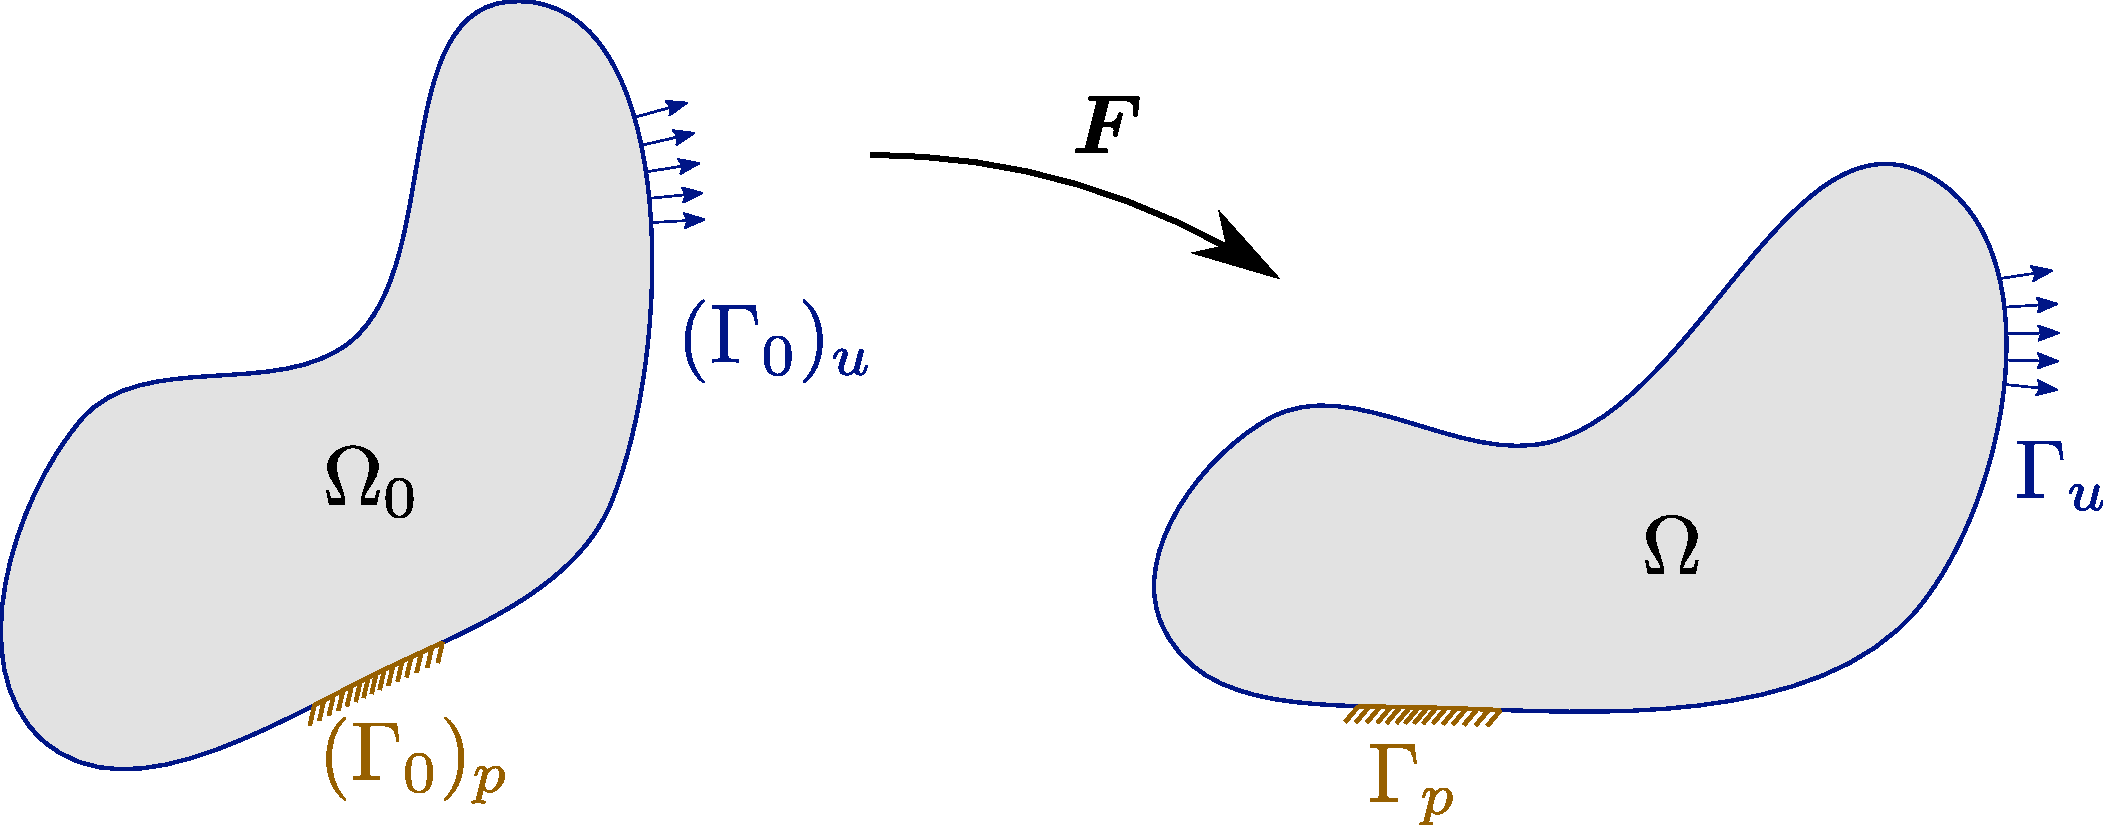
\includegraphics[width=.5\textwidth]{figures/problem.pdf}
  \caption{Generic problem definition}
  \label{fig:problem}
\end{figure}

In practice, one is not looking for the map $\vec{x} = \varphi(\vec{X},t)$, but for the deformation gradient $\bm{F}$,  or in fact for a displacement field $\vec{u} = \vec{x} - \vec{X}$. To make things a bit more explicit, the deformation gradient is defined as follows:
\begin{equation}
  \vec{x} = \bm{F} \cdot \vec{X}
\end{equation}
hence
\begin{equation}
  \bm{F}
  =
  \frac{\partial \varphi}{\partial \vec{X}}
  =
  \big( \vec{\nabla}_0 \, \vec{x} \big)^T
  =
  \bm{I} + \big( \vec{\nabla}_0 \, \vec{u} \big)^T
\end{equation}

\subsection{Momentum balance}

The momentum balance reads
\begin{equation}
\label{eq:static:momentum}
  \vec{\nabla} \cdot \bm{\sigma}(\vec{x}) = \vec{0}
  \qquad
  \vec{x} \in \Omega
\end{equation}
where $\bm{\sigma}$ is the Cauchy stress which depends on the new position $\vec{x}$ and thus on the displacement $\vec{u}$. It has been assumed that all actions are instantaneous (no inertia) and, for simplicity, that there are no body forces. Loosely speaking the interpretation of this equation is that \emph{the sum of all forces vanishes} everywhere in the domain $\Omega$.

The crux of the Finite Element Method is that this non-linear differential equation is solved in a weak sense. I.e.
\begin{equation}
\label{eq:static:int}
  \int\limits_\Omega
    \vec{\phi}(\vec{x}) \cdot \big[\, \vec{\nabla} \cdot \bm{\sigma}(\vec{x}) \,\big] \;
  \mathrm{d}\Omega
  =
  0
  \qquad
  \forall \; \vec{\phi}(\vec{x}) \in \mathbb{R}^d
\end{equation}
where $\vec{\phi}$ are test functions. For reasons that become obvious below, integration by parts is applied, which results in
\begin{equation}
\label{eq:static:weak}
  \int\limits_\Omega
    \big[\, \vec{\nabla} \vec{\phi}(\vec{x}) \,\big] : \bm{\sigma}(\vec{x}) \;
  \mathrm{d}\Omega
  =
  \int\limits_\Omega
    \vec{\nabla}
    \cdot
    \big[\, \vec{\phi}(\vec{x}) \cdot \bm{\sigma}(\vec{x}) \,\big] \;
  \mathrm{d}\Omega
  \qquad
  \forall \; \vec{\phi}(\vec{x}) \in \mathbb{R}^d
\end{equation}
In going from Eq.~\eqref{eq:static:int} to Eq.~\eqref{eq:static:weak}, use has been made of the following chain rule
\begin{equation}
  \vec{\nabla} \cdot \big[\, \vec{\phi} \cdot \bm{\sigma}^T \,\big]
  =
  \big[\, \vec{\nabla} \vec{\phi} \,\big] : \bm{\sigma}^T
  +
  \vec{\phi} \cdot \big[\, \vec{\nabla} \cdot \bm{\sigma} \,\big]
\end{equation}
Note thereby that the Cauchy stress tensor is symmetric:
\begin{equation}
  \bm{\sigma} = \bm{\sigma}^T
\end{equation}

The right-hand side of this equation can be reduced to an area integral by employing Gauss's divergence theorem:
\begin{equation}
  \int\limits_\Omega \vec{\nabla} \cdot \vec{t}(\vec{x}) \; \mathrm{d}\Omega
  =
  \int\limits_\Gamma \vec{n}(\vec{x}) \cdot \vec{t}(\vec{x}) \; \mathrm{d}\Gamma
\end{equation}
where $\vec{n}$ is the normal along the surface $\Gamma$. The result reads
\begin{equation}
\label{eq:static:weak:final}
  \int\limits_\Omega
    \big[\, \vec{\nabla} \vec{\phi}(\vec{x}) \,\big] : \bm{\sigma}(\vec{x}) \;
  \mathrm{d}\Omega
  =
  \int\limits_\Gamma
    \vec{\phi}(\vec{x}) \cdot
    \underbrace{
      \vec{n}(\vec{x}) \cdot \bm{\sigma}(\vec{x})
    }_{
      \vec{t}(\vec{x})
    } \;
  \mathrm{d}\Gamma
  \qquad
  \forall \; \vec{\phi}(\vec{x}) \in \mathbb{R}^d
\end{equation}

\subsection{Discretisation}

The problem is now discretised using $n$ \emph{nodes} that are connected through \emph{elements}, which define the discretised domain $\Omega^h_0$. Shape functions $N_i(\vec{x})$ are used to interpolate the nodal quantities throughout the domain $\Omega^h_0$ (and $\Omega^h$). For example, the discretisation and interpolation of the displacement field reads
\begin{equation}
  \vec{u}(\vec{x},t)
  \approx
  \vec{u}^h(\vec{x},t)
  =
  \sum_{m=1}^{n_\mathrm{nodes}} N_m (\vec{x}) \; \vec{u}_m (t)
\end{equation}
whereby we will not further consider the time dependence (denoted with $t$) for now. Following standard Galerkin the test functions are interpolated in the same way, i.e.\
\begin{equation}
\label{eq:discretisation}
  \vec{\phi}(\vec{x})
  \approx
  \vec{\phi}^h(\vec{x})
  =
  \sum_{m=1}^{n_\mathrm{nodes}} N_m (\vec{x}) \; \vec{\phi}_m
\end{equation}
Applied to the problem sketch from Fig.~\ref{fig:problem}, a discretisation might look like Fig.~\ref{fig:problem:discretised}. The nodes are clearly marked as circles. The lines connecting the nodes clearly mark the elements which are in this case three-node linear triangles.

\begin{figure}[htp]
  \centering
  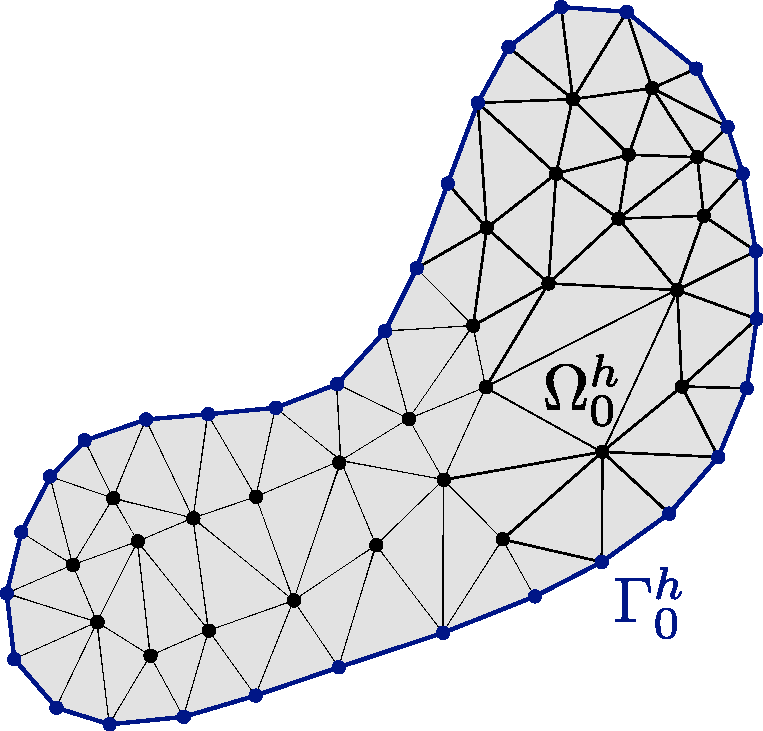
\includegraphics[width=.25\textwidth]{figures/problem-discretized.pdf}
  \caption{Example of a discretisation of the problem in Fig.~\ref{fig:problem} using Finite Elements (linear triangles in this case).}
  \label{fig:problem:discretised}
\end{figure}

Applied to the balance equation the following is obtained
\begin{equation}
  \vec{\phi}_m \cdot
  \int\limits_{\Omega^h}
    \big[\, \vec{\nabla} N_m (\vec{x}) \,\big]
    \cdot
    \bm{\sigma}(\vec{x}) \;
  \mathrm{d}\Omega
  =
  \vec{\phi}_m \cdot
  \int\limits_{\Gamma^h}
    N_m (\vec{x}) \cdot
    \vec{t}(\vec{x}) \;
  \mathrm{d}\Gamma
  \qquad
  \forall \; \vec{\phi}_m \in \mathbb{R}^d_n
\end{equation}
from which the dependency on $\vec{\phi}_m$ can be dropped:
\begin{equation}
  \int\limits_{\Omega^h}
    \big[\, \vec{\nabla} N_m (\vec{x}) \,\big]
    \cdot
    \bm{\sigma}(\vec{x}) \;
  \mathrm{d}\Omega
  =
  \int\limits_{\Gamma^h}
    N_m (\vec{x}) \cdot
    \vec{t}(\vec{x}) \;
  \mathrm{d}\Gamma
\end{equation}
This corresponds to a (non-linear) set of nodal balance equations:
\begin{equation}
  \vec{f}_m^\mathrm{int}(\vec{x})
  =
  \vec{f}_m^\mathrm{ext}(\vec{x})
\end{equation}
with:
\begin{itemize}
  \item \emph{Internal forces}
  \begin{equation}
    \vec{f}_m^\mathrm{int}(\vec{x})
    =
    \int\limits_{\Omega^h}
      \big[\, \vec{\nabla} N_m (\vec{x}) \,\big]
      \cdot
      \bm{\sigma}(\vec{x}) \;
    \mathrm{d}\Omega
  \end{equation}
  \item \emph{External forces}
  \begin{equation}
    \vec{f}_m^\mathrm{ext}(\vec{x})
    =
    \int\limits_{\Gamma^h}
      N_m (\vec{x}) \cdot
      \vec{t}(\vec{x}) \;
    \mathrm{d}\Gamma
  \end{equation}
  Note that this term is zero in the interior of the domain, i.e. in $\Omega^h \bigcap \Gamma^h$, while it can be zero or non-zero in $\Gamma^h$ depending on the problem details. Most often it follows completely from the boundary conditions of the boundary value problem that we set out to solve.
\end{itemize}

\subsection{Iterative solution -- small strain}

A commonly used strategy to solve the non-linear system is the iterative Newton-Raphson scheme (see Appendix~\ref{sec:newton-raphson}). The idea is thereby to formulate an initial guess for the solution, determine possible residual forces, and use these forces to come to a better guess for the solution. This is continued until the solution has been found, i.e. when the residual vanishes.

This solution technique is discussed here in the context of small deformations. Assuming the deformations (and therefore rotations) to be small, leads to the assumption that $\Omega = \Omega_0$, and thus that $\nabla = \nabla_0$. In this context one typically uses the linear strain tensor
\begin{equation}
  \bm{\varepsilon}
  =
  \tfrac{1}{2} \left[ \nabla_0 \vec{u} + \big[\, \nabla_0 \vec{u} \,\big]^T \right]
  =
  \mathbb{I}_s : \big[\, \nabla_0 \vec{u} \,\big]
\end{equation}
and some (non-linear) relationship between it and the stress as follows
\begin{equation}
  \bm{\sigma} = \bm{\sigma} \big( \bm{\varepsilon} \big)
\end{equation}
To further simplify the discussion, the boundary tractions are assumed to be some displacement independent quantity, which is \textit{a-priori} known for all relevant boundary nodes.

The nodal equilibrium equations now reads
\begin{equation}
\label{eq:static:eq-non-lin}
  \vec{r}_m(\vec{X}, \vec{u})
  =
  \vec{f}_m^\mathrm{ext}(\vec{X})
  -
  \vec{f}_m^\mathrm{int}(\vec{X}, \vec{u})
  =
  \underline{\vec{0}}
\end{equation}
with
\begin{equation}
  \vec{f}_m^\mathrm{int}(\vec{X}, \vec{u})
  =
  \int\limits_{\Omega^h_0}
    \big[\, \vec{\nabla}_0 N_m(\vec{X}) \,\big]
    \cdot
    \bm{\sigma}(\vec{X}, \vec{u}) \;
  \mathrm{d}\Omega_0
\end{equation}

The displacement field $\vec{u}$ is now iteratively updated starting from some initial guess, i.e.
\begin{equation}
  \vec{u}_{(i+1)} = \vec{u}_{(i)} + \delta \vec{u}
\end{equation}
The update, $\delta \vec{u}$, follows from the linearization of Eq.~\eqref{eq:static:eq-non-lin}. The results of which is
\begin{equation}
  \int\limits_{\Omega^h_0}
    \big[\, \vec{\nabla}_0 N_m(\vec{X}) \,\big]
    \cdot
    \mathbb{K}\big(\vec{X},\vec{u}_{(i)}\big)
    \cdot
    \big[\, \vec{\nabla}_0 N_n(\vec{X}) \,\big] \;
  \mathrm{d}\Omega_0
  \cdot \delta \vec{u}_n
  =
  \vec{f}_m^\mathrm{ext}(\vec{X})
  -
  \int\limits_{\Omega^h_0}
    \big[\, \vec{\nabla}_0 N_m(\vec{X}) \,\big]
    \cdot
    \bm{\sigma}\big(\vec{X},\vec{u}_{(i)}\big) \;
  \mathrm{d}\Omega_0
\end{equation}
where, at each position $\vec{X}$,
\begin{equation}
  \mathbb{K}\big(\vec{u}_{(i)}\big)
  =
  \left. \frac{\partial \bm{\sigma}}{\partial \bm{\varepsilon}} \right|_{\vec{u}_{(i)}}
  :
  \mathbb{I}_s
\end{equation}
is the \emph{constitutive tangent operator}.

In a shorter notation, the iterative update reads:
\begin{equation}
  \bm{K}_{mn,(i)} \cdot \delta \vec{u}_m
  =
  \vec{f}_m^\mathrm{ext}
  -
  \vec{f}_{m,(i)}^\mathrm{int}
\end{equation}
with
\begin{equation}
  \bm{K}_{mn,(i)}
  =
  \int\limits_{\Omega^h_0}
    \big[\, \vec{\nabla}_0 N_m(\vec{X}) \,\big]
    \cdot
    \mathbb{K}\big(\vec{X}, \vec{u}_{(i)}\big)
    \cdot
    \big[\, \vec{\nabla}_0 N_m(\vec{X}) \,\big] \;
  \mathrm{d}\Omega_0
\end{equation}
and
\begin{equation}
  \vec{f}_{m,(i)}^\mathrm{int}
  =
  \int\limits_{\Omega^h_0}
    \big[\, \vec{\nabla}_0 N_m(\vec{X}) \,\big]
    \cdot
    \bm{\sigma}\big(\vec{X}, \vec{u}_{(i)}\big) \;
  \mathrm{d}\Omega_0
\end{equation}

\subsection{Iterative solution -- large strain [work-in-progress]}

\subsubsection{Definitions}

\paragraph{Deformation gradient tensor}

Deformation gradient tensor
\begin{equation}
  \bm{F} = (\vec{\nabla}_0 \vec{x})^T
\end{equation}
The gradient operation $\vec{\nabla}$ with respect to the current configuration is related to the gradient operator with respect to the undeformed configuration $\vec{\nabla}_0$ by the deformation gradient tensor $\bm{F}$ according to
\begin{equation}
  \vec{\nabla} = \bm{F}^{-T} \cdot \vec{\nabla}_0
\end{equation}

\paragraph{Discretisation}

\begin{equation}
  \vec{x}^h (\vec{X}_0, t) = \sum\limits_{m} N_m (\vec{X}_0) \vec{x}_m (t)
\end{equation}

\subsubsection{Updated Lagrange}

Linearised system of equations:
\begin{equation}
  \int\limits_{\Omega_{(i)}^h} \vec{\nabla}_{(i)} N_m(\vec{X}_0) \cdot \big(
    \bm{F}_{(i)} \cdot \delta \bm{F}^{-1} \cdot \bm{\tau}_{(i)} + \delta \bm{\tau}
  \big) \frac{1}{J^i} d \Omega_{(i)}^h
  =
  \vec{f}_{m}^\mathrm{ext} - \vec{f}_{m,(i)}^\mathrm{int}
\end{equation}
with
\begin{equation}
  \vec{f}_{m,(i)}^\mathrm{int} = \int\limits_{\Omega_{(i)}^h} \vec{\nabla}_{(i)} N_m(\vec{X}_0) \cdot \bm{\tau}_{(i)} \frac{1}{J^i} d \Omega_{(i)}^h
\end{equation}

Introduce:
\begin{equation}
  \bm{L}_\delta
  \equiv \delta \bm{F} \cdot \bm{F}_{(i)}^{-1}
  = \left( \bm{F}_{(i)}^{-T} \cdot \delta \bm{F}^T \right)^T
  = \left( \bm{F}_{(i)}^{-T} \cdot \vec{\nabla}_0 \delta \vec{x} \right)^T
  = \left( \vec{\nabla}_{(i)} \delta \vec{x} \right)^T
\end{equation}
Hence
\begin{equation}
  \bm{L}_\delta^T \equiv \vec{\nabla}_{(i)} \delta \vec{x}
\end{equation}
and hence
\begin{equation}
  \bm{L}_\delta^T
  \equiv \vec{\nabla}_{(i)} \delta \vec{x}
  \approx \vec{\nabla}_{(i)} \delta \vec{x}^h
  = \left( \vec{\nabla}_{(i)} N_m(\vec{X}_0) \right)^T \delta \vec{x}
\end{equation}

\section{Dynamics}

\subsection{Momentum balance}

The next step is to add inertia to the balance of momentum in Eq.~\eqref{eq:static:momentum}:
\begin{equation}
  \rho\, \vec{a}
  =
  \vec{\nabla} \cdot
  \bm{\sigma}(\vec{x})
  \qquad
  \vec{x} \in \Omega
\end{equation}
where $\rho$ is the mass density, and second time derivative of the position $\vec{x}$ is the acceleration $\vec{a} = \ddot{\vec{u}} = \ddot{\vec{x}}$. Note that this function is the continuum equivalent of $\vec{f} = m \vec{a}$.

Like before, this equation is solved in a weak sense
\begin{equation}
  \int\limits_\Omega
    \rho(\vec{x})\; \vec{\phi}(\vec{x}) \cdot \vec{a} \;
  \mathrm{d}\Omega
  =
  \int\limits_\Omega
    \vec{\phi}(\vec{x})
    \cdot
    \Big[\,
      \vec{\nabla}
      \cdot
      \bm{\sigma}(\vec{x})
    \,\Big] \;
  \mathrm{d}\Omega
  \qquad
  \forall \; \vec{\phi}(\vec{x}) \in \mathbb{R}^d
\end{equation}
Integration by parts results in
\begin{equation}
  \int\limits_\Omega
    \rho(\vec{x})\; \vec{\phi}(\vec{x}) \cdot \vec{a} \;
  \mathrm{d}\Omega
  =
  \int\limits_\Gamma
    \vec{\phi}(\vec{x}) \cdot \vec{t}(\vec{x}) \;
  \mathrm{d}\Gamma
  -
  \int\limits_\Omega
    \big[\, \vec{\nabla} \vec{\phi}(\vec{x}) \,\big]
    :
    \bm{\sigma}(\vec{x}) \;
  \mathrm{d}\Omega
  \qquad
  \forall \; \vec{\phi}(\vec{x}) \in \mathbb{R}^d
\end{equation}
which is discretised as before:
\begin{equation}
  \vec{\phi}_m \cdot
  \int\limits_\Omega
    \rho(\vec{x})\; N_m(\vec{x})\; N_n(\vec{x}) \;
  \mathrm{d}\Omega \;
  \vec{a}_n
  =
  \vec{\phi}_m \cdot
  \int\limits_\Gamma
    N_m(\vec{x})\; \vec{t}(\vec{x}) \;
  \mathrm{d}\Gamma
  -
  \vec{\phi}_m \cdot
  \int\limits_\Omega
    \big[\, \vec{\nabla} N_m(\vec{x}) \,\big]
    :
    \bm{\sigma}(\vec{x}) \;
  \mathrm{d}\Omega
\end{equation}
which should still hold for all $\vec{\phi}_m \in \mathbb{R}^d_n$. However, this dependence can now trivially be dropped. Hence:
\begin{equation}
\label{eq:dynamics:system}
  \underbrace{
    \int\limits_\Omega
      \rho(\vec{x})\; N_m(\vec{x})\; N_n(\vec{x}) \;
    \mathrm{d}\Omega
  }_{\displaystyle
    M_{mn}(\vec{x})
  } \;
  \vec{a}_n
  =
  \underbrace{
    \int\limits_\Gamma
      N_m(\vec{x})\; \vec{t}(\vec{x}) \;
    \mathrm{d}\Gamma
  }_{\displaystyle
    \vec{f}_m^\mathrm{ext}(\vec{x})
  }
  -
  \underbrace{
    \int\limits_\Omega
      \big[\, \vec{\nabla} N_m(\vec{x}) \,\big]
      :
      \bm{\sigma}(\vec{x}) \;
    \mathrm{d}\Omega
  }_{\displaystyle
    \vec{f}_m^\mathrm{int}(\vec{x})
  }
\end{equation}
This is denoted as follows
\begin{equation}
  M_{mn}(\vec{x})\; \vec{a}_n
  =
  \vec{f}_m^\mathrm{ext}(\vec{x})
  -
  \vec{f}_m^\mathrm{int}(\vec{x})
\end{equation}
Where $M_{mn}(\vec{x})$ is the \emph{mass matrix}, $\vec{f}_m^\mathrm{ext}(\vec{x})$ are the \emph{external forces}, and $\vec{f}_m^\mathrm{int}(\vec{x})$ are the \emph{internal forces}.

\subsection{Time discretisation}
\label{eq:dynamics:time}

To solve the second order differential equation in time, one typically also discretises time with some finite difference based scheme. For this we also need to distinguish the velocity field $\vec{v} = \dot{\vec{u}} = \dot{\vec{x}}$.

\subsubsection{Verlet}

In the case that the forces are velocity independent one can use the Velocity Verlet scheme, in which energy is conserved, i.e.\ it is reversible in time. The scheme reads as follows:

\begin{enumerate}
  \item Compute the velocity on a dummy time grid:
  \begin{equation}
    \vec{v}_{n+1/2} = \vec{v}_{n-1/2} + \Delta_t \; \vec{a}_n
  \end{equation}
  Note that this involves solving Eq.~\eqref{eq:dynamics:system} for $\vec{a}_n$. From this it is directly obvious why the forces need to be velocity independent.
  \item Update the positions
  \begin{equation}
    \vec{u}_{n+1} = \vec{u}_n + \Delta_t \;\vec{a} \vec{v}_{n + 1/2}
  \end{equation}
\end{enumerate}

\subsubsection{Velocity Verlet}

In the case that the forces are dependent on the velocity (i.e.\ when there is damping) the previous scheme cannot be used anymore. An additional approximation has to be made in this case. Note that this is not very problematic as energy is in no case conserved. The resulting scheme reads:

\begin{enumerate}
  \item Compute the position at $t_{n+1} = t_{n} + \Delta_t$:
  \begin{equation}
    \vec{u}_{n+1}
    =
    \vec{u}_{n} + \Delta_t \vec{v}_{n} + \tfrac{1}{2} \Delta_t^2 \vec{a}_{n}
  \end{equation}
  \item Estimate the velocity at $t_{n+1} = t_{n} + \Delta_t$ (involves solving Eq.~\eqref{eq:dynamics:system}):
  \begin{equation}
    \hat{\vec{v}}_{n+1}
    =
    \vec{v}_{n}
    +
    \tfrac{1}{2} \Delta_t \Big[\,
      \vec{a}_{n} + \vec{a} ( \vec{u}_{n+1} , \vec{v}_{n} + \Delta_t \vec{a}_{n} , t_{n+1} ) \,
    \Big]
  \end{equation}
  \item Correct $\hat{\vec{v}}_{n+1}$ (involves solving Eq.~\eqref{eq:dynamics:system}):
  \begin{equation}
    \vec{v}_{n+1}
    =
    \vec{v}_{n}
    +
    \tfrac{1}{2} \Delta_t \Big[\,
      \vec{a}_{n} + \vec{a} ( \vec{u}_{n+1} , \hat{\vec{v}}_{n+1} , t_{n+1} ) \,
    \Big]
  \end{equation}
\end{enumerate}

\subsection{Approximations}

For problems where the local volume is conversed (either weakly through slightly compressible elasticity, or strongly by adding an incompressibility constraint) it makes sense to assume the mass matrix constant, as any change of volume results in an equivalent change of the density. In that case
\begin{equation}
  \int\limits_{\Omega}
    \rho(\vec{x})
  \;\mathrm{d}\Omega
  =
  \int\limits_{\Omega_0}
    \rho(\vec{X})
  \;\mathrm{d}\Omega_0
\end{equation}
Which results in:
\begin{equation}
  M_{mn}(\vec{x})
  =
  \int\limits_{\Omega_0}
    \rho(\vec{X})\; N_m(\vec{X})\; N_n(\vec{X}) \;
  \mathrm{d}\Omega_0
  =
  \mathrm{constant}
\end{equation}

To enhance computational efficiency, it may be a good option concentrate the mass to point masses on the nodes. This has to strong advantage that the mass matrix becomes diagonal, known as the \emph{lumped mass matrix}. Consequently, instead of solving a linear system one just has to solve fully independent equations.

\appendix

\section{Nomenclature}

\begin{itemize}
  \item Vector
  \begin{equation}
    \vec{u} = \sum\limits_i u_i \vec{e}_i
  \end{equation}
  for example for Cartesian coordinates
  \begin{equation}
    \vec{u} = u_x \vec{e}_x + u_y \vec{e}_y + u_z \vec{e}_z
  \end{equation}
  %
  \item Second-order tensor
  \begin{equation}
    \bm{A} = \sum\limits_i \sum\limits_j A_{ij} \vec{e}_i \vec{e}_j
  \end{equation}
  %
  \item Fourth-order tensor
  \begin{equation}
    \mathbb{A} = \sum\limits_i \sum\limits_j \sum\limits_k \sum\limits_l A_{ijkl} \vec{e}_i \vec{e}_j \vec{e}_k \vec{e}_l
  \end{equation}
  %
  \item Divergence
  \begin{equation}
    \vec{\nabla} \cdot \bm{\sigma} = \frac{ \partial \sigma_{ij} }{ \partial x_i }
  \end{equation}
  %
  \item Double tensor contraction
  \begin{equation}
    C = \bm{A} : \bm{B} = A_{ij} B_{ji}
  \end{equation}
\end{itemize}

\section{Shape functions}

In the Finite Element Method a geometry is discretised using nodes. The nodes are grouped in elements which define the domain $\Omega^h$. The crux of the method is that nodal quantities, for example $\vec{u}_m$, are interpolated throughout the discretised domain $\Omega^h$ using shape functions $N_m (\vec{x})$. The shape functions are polynomials that spanned by the nodes, such that they constitute a partition of unity and satisfy $N_m (\vec{x}_n) = \delta_{mn}$, i.e. it is one in the node $i$, and zero in all other nodes. This implies that, while each shape function is globally supported, $N_m (\vec{x}) \neq 0$ only in the elements containing node $i$. For all other elements it is zero (even in between the nodes). This again implies that $\partial N_m / \partial \vec{x}$ is discontinuous across element boundaries.

For a one-dimensional problem comprising four linear elements and five nodes, the shape functions are sketched in Fig.~\ref{fig:shape:1d-domain}. To emphasise the global support of each shape function the shape function of node 2 is isolated in Fig.~\ref{fig:shape:1d-domain-2}. As can be seen, node 2 is only non-zero in elements 1 and 2, while it is zero everywhere else. To evaluate for example $f_2$, the internal force one node 2, the integration can be limited to these two elements:
\begin{equation}
  f_2
  =
  \int\limits_{\Omega^{(1)}}
    \frac{\mathrm{d} N^{(1)}_2}{\mathrm{d} x} \;
    \sigma (x) \;
  \mathrm{d}\Omega^{(1)}
  +
  \int\limits_{\Omega^{(2)}}
    \frac{\mathrm{d} N^{(2)}_2}{\mathrm{d} x} \;
    \sigma (x) \;
  \mathrm{d}\Omega^{(2)}
\end{equation}

\begin{figure}[htp]
  \centering
  \captionsetup[subfigure]{justification=centering}
  \begin{minipage}[t]{.5\textwidth}
    \centering
    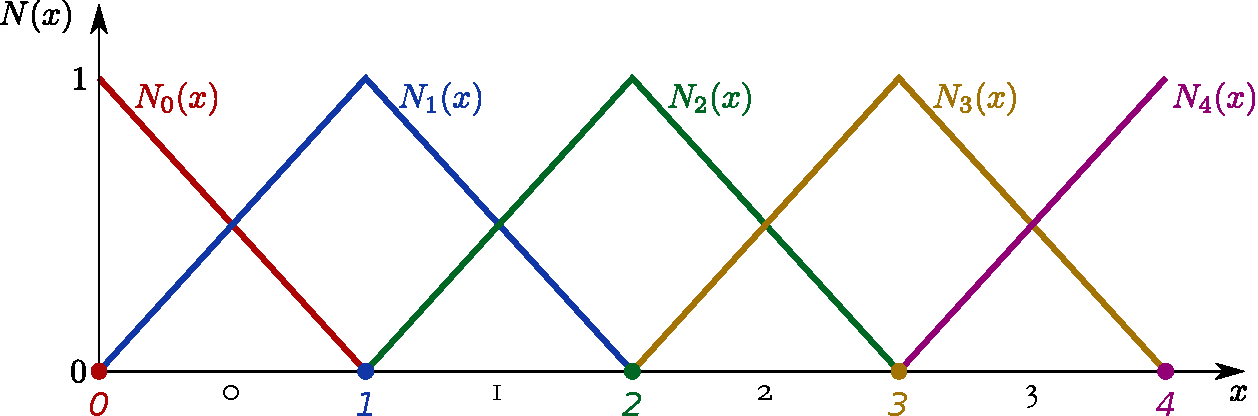
\includegraphics[width=1.\textwidth]{figures/shape-functions-1d.pdf}
    \subcaption{All shape functions $N_m(x)$, each with a different colour.}
    \label{fig:shape:1d-domain}
  \end{minipage}
  \\
  \begin{minipage}[t]{.5\textwidth}
    \centering
    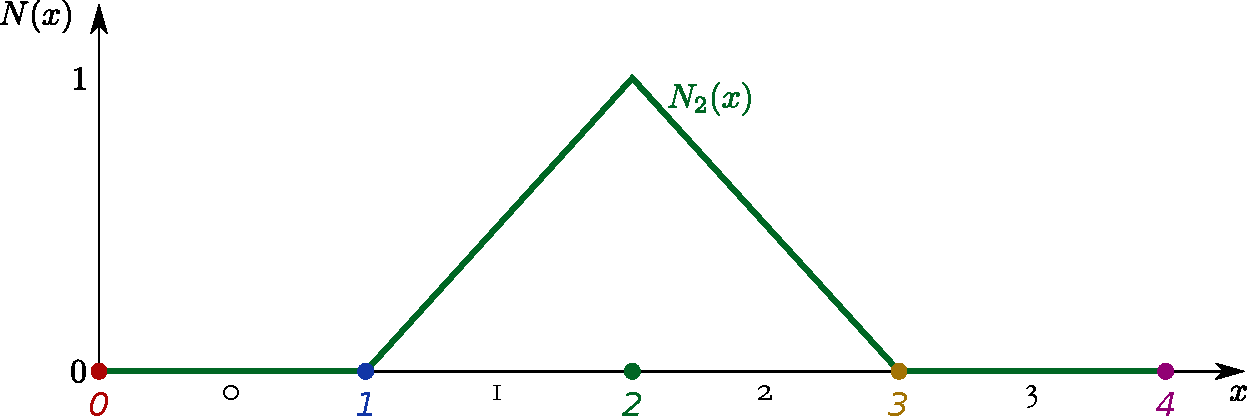
\includegraphics[width=1.\textwidth]{figures/shape-functions-1d-node-2.pdf}
    \subcaption{Isolated shape function $N_2(x)$.}
    \label{fig:shape:1d-domain-2}
  \end{minipage}
  \caption{(a) Shape functions for a one-dimensional domain discretised using four two node, linear, element. (b) Isolated shape functions for node 2. The node numbers are displayed using a unique colour, while the element numbers are shown in black in a different font, in between the nodes.}
  \label{fig:shape:1d-domain:fig}
\end{figure}

By now it should be clear that the above allows the global system $f_m$ to be assembled element-by-element. For the example in Fig.~\ref{fig:shape:1d-domain:fig} this is graphically shown in Fig.~\ref{fig:shape:1d-domain:assembly} where the indices show that the \emph{shape functions} are evaluated compared to some generic element definition.

\begin{figure}[htp]
  \centering
  \captionsetup[subfigure]{justification=centering}
  \begin{minipage}[t]{.5\textwidth}
    \centering
    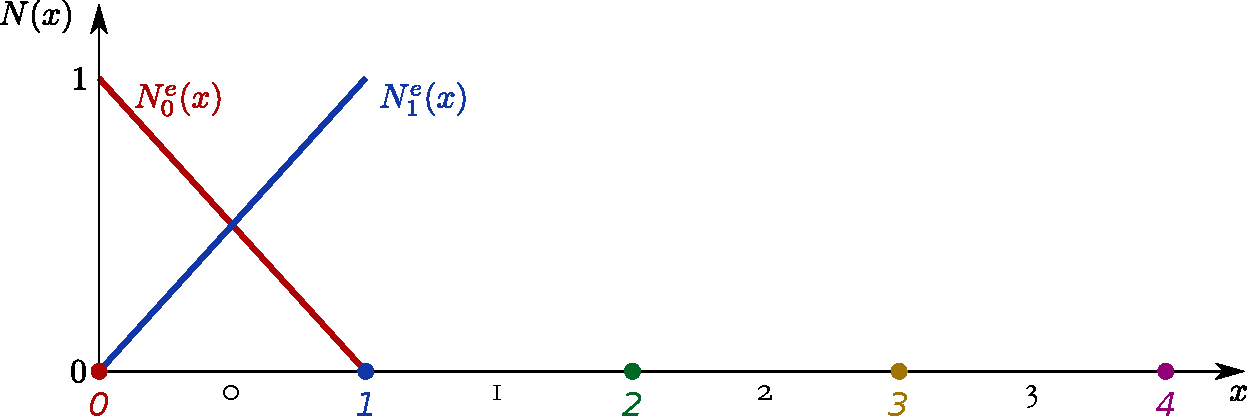
\includegraphics[width=1.\textwidth]{figures/shape-functions-1d-element-0.pdf}
  \end{minipage}
  \\
  $+$
  \\
  \begin{minipage}[t]{.5\textwidth}
    \centering
    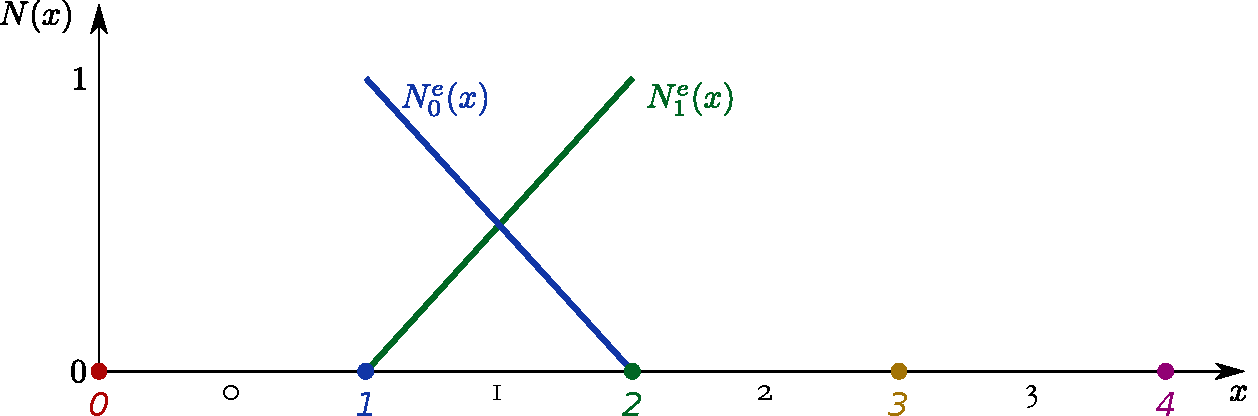
\includegraphics[width=1.\textwidth]{figures/shape-functions-1d-element-1.pdf}
  \end{minipage}
  \\
  $+$
  \\
  \begin{minipage}[t]{.5\textwidth}
    \centering
    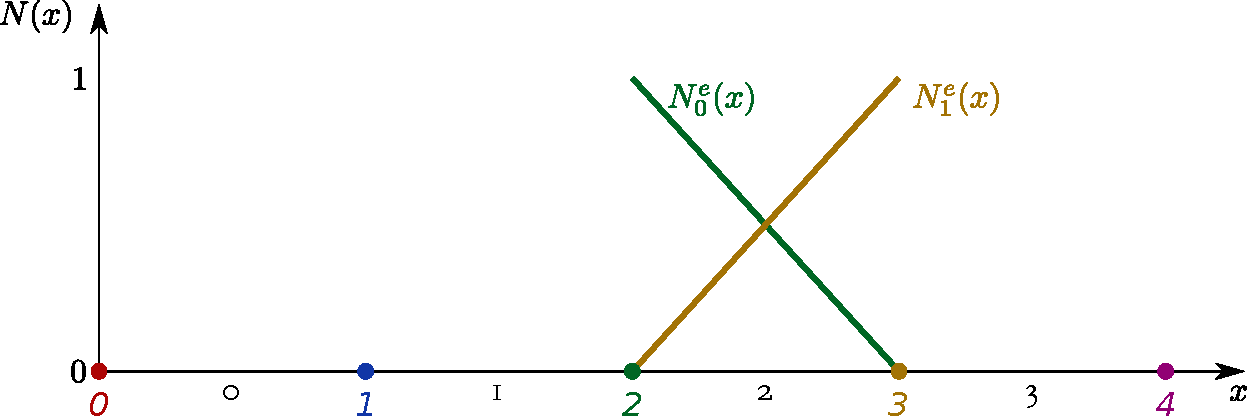
\includegraphics[width=1.\textwidth]{figures/shape-functions-1d-element-2.pdf}
  \end{minipage}
  \\
  $+$
  \\
  \begin{minipage}[t]{.5\textwidth}
    \centering
    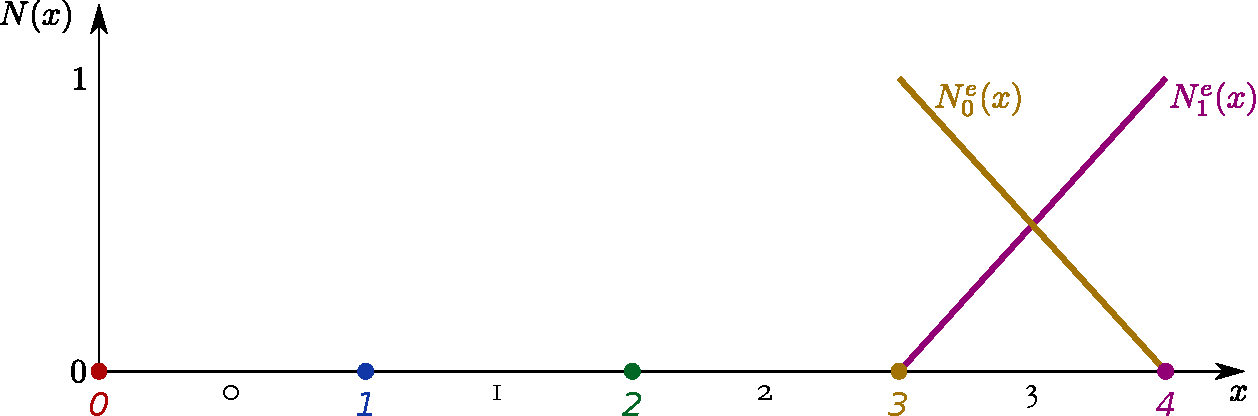
\includegraphics[width=1.\textwidth]{figures/shape-functions-1d-element-3.pdf}
  \end{minipage}
  \caption{Element-by-element assembly of the problem in Fig.~\ref{fig:shape:1d-domain:fig}.}
  \label{fig:shape:1d-domain:assembly}
\end{figure}

\section{Iso-parametric transformation and quadrature}

A very important concept in the Finite Element Method is the iso-parametric transformation. It allows an arbitrarily shaped element with volume $\Omega^e$ to be mapped onto a generic \emph{iso-parametric element} of constant volume $Q$, see Fig.~\ref{fig:isoparametric}. Using this mapping it is easy to perform interpolation and numerical quadrature using a generic implementation.

\begin{figure}[htp]
  \centering
  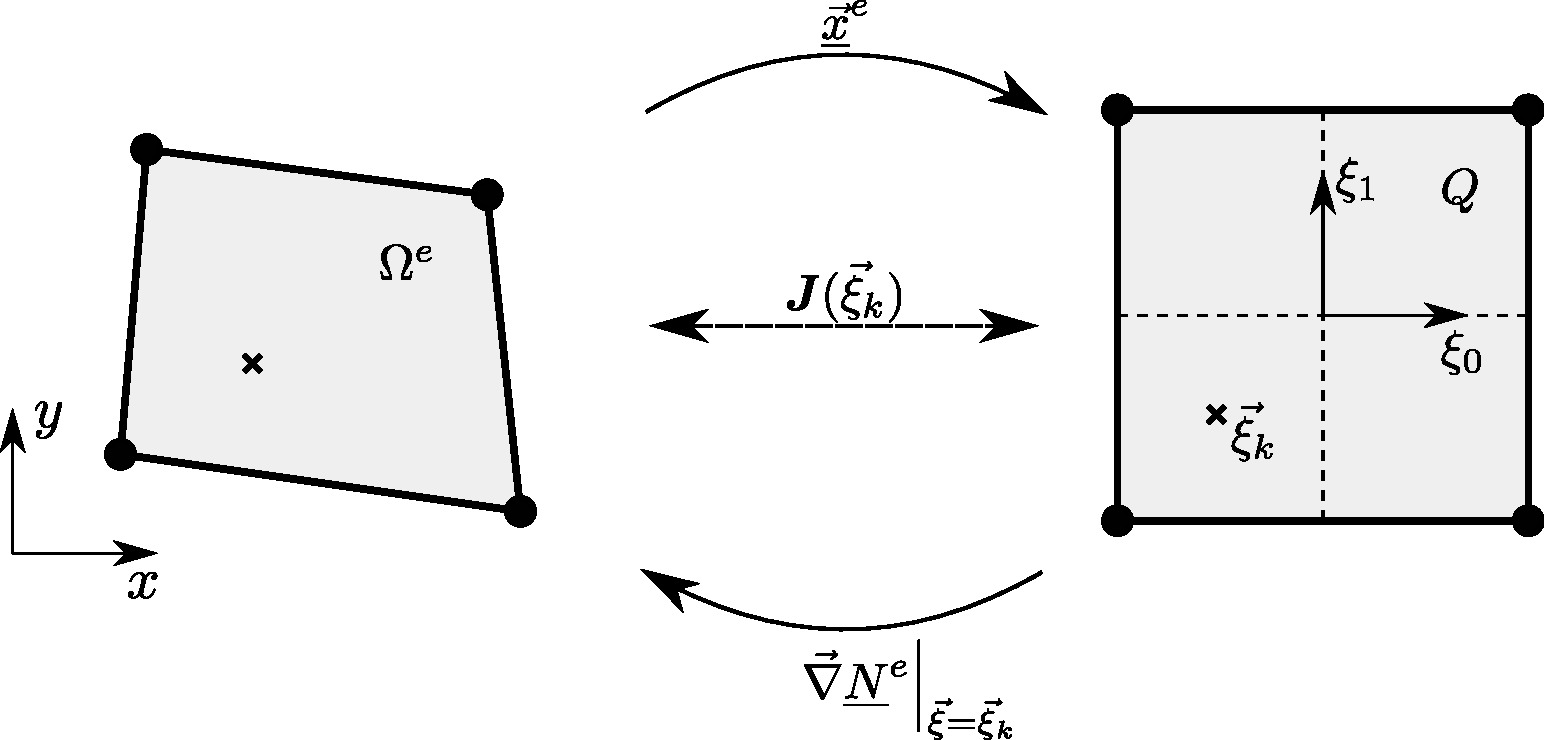
\includegraphics[width=.5\textwidth]{figures/isoparametric-transform.pdf}
  \caption{Iso-parametric transformation for a four node, bi-linear, quadrilateral element.}
  \label{fig:isoparametric}
\end{figure}

The mapping between the generic domain $Q$ and the physical domain $\Omega^e$ is as follows
\begin{equation}
\label{eq:isoparametric:coordinate}
  \vec{x} ( \vec{\xi} ) = N_m^{e} \; \vec{x}_m^e
\end{equation}
where the column $\vec{x}_m^e$ contains the position vectors of the element nodes in the actual coordinates (i.e.\ spanning $\Omega^e$). In order to perform the quadrature on $Q$ we must also map the gradient operator:
\begin{equation}
  \vec{\nabla}_{\xi}\,
  =
  \vec{e}_i \frac{\partial}{\partial \xi_i}
  =
  \vec{e}_i \frac{\partial x_j(\vec{\xi})}{\partial \xi_i} \frac{\partial}{\partial x_j}
  =
  \vec{e}_i \frac{\partial x_j(\vec{\xi})}{\partial \xi_i} \vec{e}_j \cdot \vec{e}_k \frac{\partial}{\partial x_k}
  =
  \big[\, \vec{\nabla}_{\xi}\, \vec{x}(\vec{\xi}) \,\big] \cdot \vec{\nabla}
  =
  \bm{J}(\vec{\xi}) \cdot \vec{\nabla}
\end{equation}
i.e.
\begin{equation}
  J_{ij} = \frac{\partial x_i}{\partial \xi_j}
\end{equation}
from which the inverse relationship trivially follows
\begin{equation}
  \vec{\nabla} = \bm{J}^{-1}(\vec{\xi}) \cdot \vec{\nabla}_{\xi}\,
\end{equation}
where $\bm{J}$ is the Jacobian which can be obtained from the gradient of the shape functions with respect to the iso-parametric coordinates and the nodal coordinates in the actual coordinates through Eq.~\eqref{eq:isoparametric:coordinate}:
\begin{equation}
  \bm{J}(\vec{\xi})
  =
  \vec{\nabla}_{\xi}\, \vec{x}(\vec{\xi})
  =
  \vec{\nabla}_{\xi}\, \big[\, N_m^{e} \; \vec{x}_m^e \,\big]
  =
  \big[\, \vec{\nabla}_{\xi}\, N_m^{e} \,\big] \; \vec{x}_m^e
\end{equation}

The gradient of the shape functions with respect to the actual coordinates can now be computed though
\begin{equation}
  \vec{\nabla} N_m^{e}
  =
  \bm{J}^{-1}(\vec{\xi}) \cdot  \big[\, \vec{\nabla}_{\xi}\, N_m^{e} \,\big]
\end{equation}

The change of variables should also be accounted for in the integration:
\begin{equation}
  \int_\Omega (\ldots) \; \mathrm{d} \Omega
  =
  \iiint (\ldots) \; \mathrm{d} x \, \mathrm{d} y \, \mathrm{d} z
  =
  \iiint (\ldots) \; \left| \frac{\partial \left( x, y, z \right)}{\partial \left( \xi, \eta, \mu \right)} \right| \mathrm{d} \xi \, \mathrm{d} \eta \, \mathrm{d} \mu
\end{equation}
where the determinant of the Jacobian
\begin{equation}
  \frac{\partial \left( x, y, z \right)}{\partial \left( \xi, \eta, \mu \right)}
  =
  \left|
    \begin{array}{ccc}
      \displaystyle \frac{\partial x}{\partial \xi } &
      \displaystyle \frac{\partial x}{\partial \eta} &
      \displaystyle \frac{\partial x}{\partial \mu }
      \\
      \displaystyle \frac{\partial y}{\partial \xi } &
      \displaystyle \frac{\partial y}{\partial \eta} &
      \displaystyle \frac{\partial y}{\partial \mu }
      \\
      \displaystyle \frac{\partial z}{\partial \xi } &
      \displaystyle \frac{\partial z}{\partial \eta} &
      \displaystyle \frac{\partial z}{\partial \mu }
    \end{array}
  \right|
\end{equation}
We can now make use of the Jacobian that we already obtained
\begin{equation}
  \int_\Omega (\ldots) \; \mathrm{d} \Omega
  =
  \iiint (\ldots) \det \left( \bm{J}(\vec{\xi}) \right) \; \mathrm{d} \xi \, \mathrm{d} \eta \, \mathrm{d} \mu
  =
  \int_Q (\ldots) \det \left( \bm{J}(\vec{\xi}) \right) \; \mathrm{d} Q
\end{equation}
Note that another way to obtain this result is using
\begin{align}
  \mathrm{d} \Omega
  &=
  \mathrm{d} \vec{x}_0 \times \mathrm{d} \vec{x}_1 \cdot \mathrm{d} \vec{x}_2
  =
  \left[ \mathrm{d} \vec{x}_0 \cdot \bm{J}(\vec{\xi}) \right] \times
  \left[ \mathrm{d} \vec{x}_1 \cdot \bm{J}(\vec{\xi}) \right] \cdot
  \left[ \mathrm{d} \vec{x}_2 \cdot \bm{J}(\vec{\xi}) \right]
  =
  \det \big( \bm{J}(\vec{\xi}) \big)\,
  \mathrm{d} \vec{\xi}_0 \times \mathrm{d} \vec{\xi}_1 \cdot \mathrm{d} \vec{\xi}_2
  \\
  &=
  \det \big( \bm{J}(\vec{\xi}) \big)\, \mathrm{d} Q
\end{align}
Numerical quadrature can be formulated (exactly) on the master element. It corresponds to taking the weighted sum of the integrand evaluated at specific \emph{quadrature points} (or \emph{integration points}). The practical implications, for example for the internal force, are as follows:
\begin{align}
  \vec{f}_m^e
  &=
  \int\limits_{\Omega^e}
    \big[\, \vec{\nabla} N_m \,\big]
    \cdot
    \bm{\sigma}(\vec{x}) \;
  \mathrm{d}\Omega
  =
  \int\limits_{Q}
    \big[\, \vec{\nabla} N_m \,\big]
    \cdot
    \bm{\sigma}(\vec{x}) \;
    \det \big( \bm{J}(\vec{\xi}) \big) \;
  \mathrm{d}Q
  \\
  &=
  \sum_{k}^{n_k}
  w_k
  \big[\, \vec{\nabla} N_m \,\big]_{\vec{\xi} = \vec{\xi}_k}
  \cdot
  \bm{\sigma}\big(\vec{x}(\vec{\xi}_k)\big) \;
  \det \big( \bm{J}(\vec{\xi}_k) \big) \;
\end{align}

\subsection*{Total Lagrange}

To obtain
\begin{equation}
 \vec{x}(\vec{\xi}),\, \vec{\nabla}_0,\,\, \text{and}\, \int\limits_{\Omega_0} (\ldots) \;\mathrm{d}\Omega
\end{equation}
simply replace $\vec{x}_m^e$ with $\vec{X}_m^e$ in Eq.~\eqref{eq:isoparametric:coordinate}. For this reason the same element implementation can be used in small strain and finite strain (total Lagrange and updated Lagrange), by providing either $\vec{X}_m^e$ or $\vec{X}_m^e + \vec{u}_m^e$ as input.


\section{Newton-Raphson in one dimension}
\label{sec:newton-raphson}

The objective is to find $x$ such that
\begin{equation}
  r(x) = 0
\end{equation}
An initial guess is made for $x$ which is (hopefully) iteratively improved. This iterative value is denoted using $x_{(i)}$. It is updated by making use of the following Taylor expansion
\begin{equation}
  r \big( x_{(i+1)} \big)
  =
  r \big( x_{(i)} \big)
  +
  \left. \frac{\mathrm{d} r}{\mathrm{d} x} \right|_{x = x_{(i)}} \delta x
  +
  \mathcal{O} \big( \delta x^2 \big)
  \approx
  0
\end{equation}
where
\begin{equation}
  \delta x = x_{(i+1)} - x_{(i)}
\end{equation}
The value of $\delta x$ can be obtained by neglecting higher order terms:
\begin{equation}
  r \big( x_{(i)} \big)
  +
  \left. \frac{\mathrm{d} r}{\mathrm{d} x} \right|_{x = x_{(i)}} \delta x
  =
  0
\end{equation}
From which it follows that
\begin{equation}
  \delta x
  =
  - \left[ \left. \frac{\mathrm{d} r}{\mathrm{d} x} \right|_{x = x_{(i)}} \right]^{-1}
  r \big( x_{(i)} \big)
\end{equation}
Thereafter, the improved `guess' of the solution is
\begin{equation}
  x_{(i+1)} = x_{(i)} + \delta x
\end{equation}
These steps are then repeated, until the solution has been reached within a certain accuracy $\epsilon$:
\begin{equation}
  \left| r \big( x_{(i+1)} \big) \right| < \epsilon
\end{equation}
The iterative scheme is well understood from the illustration in Fig.~\ref{fig:newton-raphson}.

\begin{figure}[htp]
  \centering
  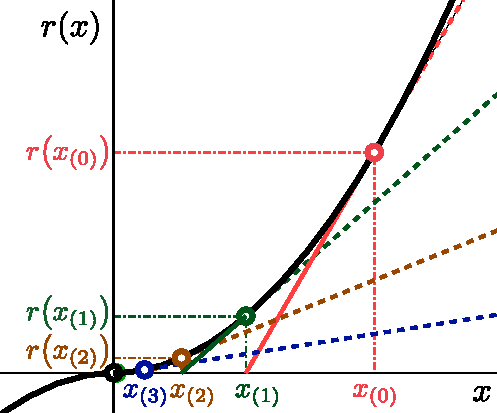
\includegraphics[width=.4\textwidth]{figures/newton-raphson.pdf}
  \caption{Schematic of the Newton-Raphson iterations in a one-dimensional problem.}
  \label{fig:newton-raphson}
\end{figure}

\section{B-matrix}

\subsection{Discretisation}

The discretisation from Eq.~\eqref{eq:discretisation} can be written more precisely as
\begin{equation}
  \phi_x(\vec{x}) \vec{e}_x +
  \phi_y(\vec{x}) \vec{e}_y +
  \phi_z(\vec{x}) \vec{e}_z
  \approx
  \sum_{m=1}^{n_\mathrm{nodes}}
  N_m (\vec{x}) \; \phi_{m,x} \vec{e}_x +
  N_m (\vec{x}) \; \phi_{m,y} \vec{e}_y +
  N_m (\vec{x}) \; \phi_{m,z} \vec{e}_z
\end{equation}
whereby $\vec{\phi}(\vec{x})$ is a vector field such as the test functions, the displacement, the forces, etc. The resulting shape function gradients then read
\begin{align}
  &
  \vec{\nabla} \vec{\phi}(\vec{x})
  \approx
  \sum_{m=1}^{n_\mathrm{nodes}}
  \bigg(
    \vec{e}_x \frac{\partial}{\partial x} +
    \vec{e}_y \frac{\partial}{\partial y} +
    \vec{e}_z \frac{\partial}{\partial z}
  \bigg)
  \bigg(
    N_m (\vec{x}) \; \phi_{m,x} \vec{e}_x +
    N_m (\vec{x}) \; \phi_{m,y} \vec{e}_y +
    N_m (\vec{x}) \; \phi_{m,z} \vec{e}_z
  \bigg)
  \\
  &
  =
  \phi_{m,x} \frac{\partial N_m}{\partial x} \vec{e}_x \vec{e}_x + \nonumber
  \phi_{m,y} \frac{\partial N_m}{\partial x} \vec{e}_x \vec{e}_y + \nonumber
  \phi_{m,z} \frac{\partial N_m}{\partial x} \vec{e}_x \vec{e}_z
  \\
  &
  +
  \phi_{m,x} \frac{\partial N_m}{\partial y} \vec{e}_y \vec{e}_x +
  \phi_{m,y} \frac{\partial N_m}{\partial y} \vec{e}_y \vec{e}_y +
  \phi_{m,z} \frac{\partial N_m}{\partial y} \vec{e}_y \vec{e}_z
  \\
  &
  +
  \phi_{m,x} \frac{\partial N_m}{\partial z} \vec{e}_z \vec{e}_x +
  \phi_{m,y} \frac{\partial N_m}{\partial z} \vec{e}_z \vec{e}_y +
  \phi_{m,z} \frac{\partial N_m}{\partial z} \vec{e}_z \vec{e}_z
\end{align}
Which can denote in short as
\begin{equation}
\label{eq:bmatrix:discretisation}
  \vec{\nabla} \vec{\phi} (\vec{x})
  \approx
  \sum_{m=1}^{n_\mathrm{nodes}}
  \mathcal{B}_m (\vec{x}) \cdot \vec{\phi}_m
\end{equation}
whereby $\mathcal{B}_m$ is third order tensor that collects the gradient of the shape function of a node $m$. The only non-zero components are
\begin{alignat}{3}
  \mathcal{B}_{m,x x x} &= \frac{\partial N_m}{\partial x} & \qquad
  \mathcal{B}_{m,y x x} &= \frac{\partial N_m}{\partial y} & \qquad
  \mathcal{B}_{m,z x x} &= \frac{\partial N_m}{\partial z}
  \nonumber
  \\
  \mathcal{B}_{m,x y y} &= \frac{\partial N_m}{\partial x}  & \qquad
  \mathcal{B}_{m,y y y} &= \frac{\partial N_m}{\partial y}  & \qquad
  \mathcal{B}_{m,z y y} &= \frac{\partial N_m}{\partial z}
  \\
  \mathcal{B}_{m,x z z} &= \frac{\partial N_m}{\partial x}  & \qquad
  \mathcal{B}_{m,y z z} &= \frac{\partial N_m}{\partial y}  & \qquad
  \mathcal{B}_{m,z z z} &= \frac{\partial N_m}{\partial z}
\end{alignat}

\subsection{Applied to the weak form}

By means of example the organisation using the `B-matrix' can be applied to the weak form of Eq.~\eqref{eq:static:weak:final}, which reads
\begin{equation}
  \int\limits_\Omega
    \big[\, \vec{\nabla} \vec{\phi}(\vec{x}) \,\big] : \bm{\sigma}(\vec{x}) \;
  \mathrm{d}\Omega
  =
  \int\limits_\Gamma
    \vec{\phi}(\vec{x}) \cdot
    \vec{t}(\vec{x}) \;
  \mathrm{d}\Gamma
  \qquad
  \forall \; \vec{\phi}(\vec{x}) \in \mathbb{R}^d
\end{equation}
Substituting Eq.~\eqref{eq:bmatrix:discretisation} results in
\begin{equation}
  \int\limits_{\Omega^h}
    \left( \mathcal{B}_m \cdot \vec{\phi}_m \right) : \bm{\sigma}(\vec{x}) \;
  \mathrm{d}\Omega
  =
  \int\limits_{\Gamma^h}
    N_m (\vec{x}) \; \vec{\phi}_m \cdot \vec{t}(\vec{x}) \;
  \mathrm{d}\Gamma
  \qquad
  \forall \; \vec{\phi}_m \in \mathbb{R}^d_n
\end{equation}
from which we can take the nodal values of the test functions $\vec{\phi}_m$, that no longer depend on space, out of the volume integral:
\begin{equation}
  \vec{\phi}_m \cdot
  \int\limits_{\Omega^h}
    \mathcal{B}_m^T : \bm{\sigma}(\vec{x}) \;
  \mathrm{d}\Omega
  =
  \vec{\phi}_m \cdot
  \int\limits_{\Gamma^h}
    N_m(\vec{x}) \; \vec{t}(\vec{x}) \;
  \mathrm{d}\Gamma
  \qquad
  \forall \; \vec{\phi}_m \in \mathbb{R}^d_n
\end{equation}
From which it is obvious that the dependence on $\vec{\phi}_m$ can be dropped, resulting in the discretised weak form:
\begin{equation}
\label{eq:bmatrix:weak_form:discrete}
  \int\limits_{\Omega^h}
    \mathcal{B}_m^T : \bm{\sigma}(\vec{x}) \;
  \mathrm{d}\Omega
  =
  \int\limits_{\Gamma^h}
    N_m(\vec{x}) \; \vec{t}(\vec{x}) \;
  \mathrm{d}\Gamma
\end{equation}

\subsection{Applied to linear elasticity}

As a further illustration linear elasticity can be assumed. Application to Eq.~\eqref{eq:bmatrix:weak_form:discrete} trivially results in
\begin{equation}
  \int\limits_{\Omega_0^h}
    \tilde{\mathcal{B}}_m^T : \Big( \mathbb{C} : \bm{\varepsilon}(\vec{x}) \Big) \;
  \mathrm{d}\Omega
  =
  \int\limits_{\Gamma^h}
    N_m(\vec{x}) \; \vec{t}(\vec{x}) \;
  \mathrm{d}\Gamma
\end{equation}
where $\tilde{\cdot}$ emphasises that $\tilde{\mathcal{B}}_m$ are the gradients of the shape functions with respect to the coordinates in the, undeformed, reference frame. Now, because $\mathbb{C}$ symmetrises, this expression can be written in terms of the displacement gradient directly:
\begin{equation}
  \int\limits_{\Omega_0^h}
    \tilde{\mathcal{B}}_m^T : \Big( \mathbb{C} : \vec{\nabla}\vec{u}(\vec{x}) \Big) \;
  \mathrm{d}\Omega
  =
  \int\limits_{\Gamma^h}
    N_m(\vec{x}) \; \vec{t}(\vec{x}) \;
  \mathrm{d}\Gamma
\end{equation}
The displacement gradient is evaluated discretely using Eq.~\eqref{eq:bmatrix:weak_form:discrete}, resulting in:
\begin{equation}
  \int\limits_{\Omega_0^h}
    \tilde{\mathcal{B}}_m^T : \Big( \mathbb{C} : ( \tilde{\mathcal{B}}_n \cdot \vec{u}_n) \Big) \;
  \mathrm{d}\Omega
  =
  \int\limits_{\Gamma^h}
    N_m(\vec{x}) \; \vec{t}(\vec{x}) \;
  \mathrm{d}\Gamma
\end{equation}
whereby, again, the nodal displacements, $\vec{u}_n$, are not a function of the position and can be taken out of the integral, such as to finally have a system that can be solved:
\begin{equation}
  \int\limits_{\Omega_0^h}
    \tilde{\mathcal{B}}_m^T : \Big( \mathbb{C} : \tilde{\mathcal{B}}_n \Big) \;
  \mathrm{d}\Omega
  \cdot \vec{u}_n
  =
  \int\limits_{\Gamma^h}
    N_m(\vec{x}) \; \vec{t}(\vec{x}) \;
  \mathrm{d}\Gamma
\end{equation}

\section{Cylindrical coordinates}

\paragraph{Coordinates}

The cylindrical coordinate system is spanned by $(\vec{e}_r, \vec{e}_\theta, \vec{e}_z)$ as visualised in Fig.~\ref{fig:cylindrical}. From this figure, the transition from cylindrical coordinates to Cartesian coordinates trivially follows to read
\begin{equation}
  x = r \cos \theta \qquad
  y = r \sin \theta \qquad
  z = z
\end{equation}
and the inverse relation to read
\begin{equation}
  r      = \sqrt{ x^2 + y^2 }                \qquad
  \theta = \mathrm{arctan}\left( y/x \right) \qquad
  z      = z
\end{equation}
Likewise, the unit vectors $(\vec{e}_r, \vec{e}_\theta, \vec{e}_z)$ can be expressed in terms of the unit vectors that span the Cartesian basis:
\begin{align}
  \vec{e}_r      &=   \cos \theta \; \vec{e}_x + \sin \theta \; \vec{e}_y \nonumber \\
  \vec{e}_\theta &= - \sin \theta \; \vec{e}_x + \cos \theta \; \vec{e}_y \nonumber \\
  \vec{e}_z      &= \vec{e}_z \label{eq:cylindrical:unit}
\end{align}
The gradient operator for cylindrical coordinates reads
\begin{equation}
  \vec{\nabla} =
  \vec{e}_r \frac{\partial}{\partial r} +
  \frac{1}{r} \vec{e}_\theta \frac{\partial}{\partial \theta} +
  \vec{e}_z \frac{\partial}{\partial z}
\end{equation}
whereby from Eq.~\eqref{eq:cylindrical:unit} the derivates of the unit vector follow to be
\begin{alignat}{3}
  \frac{\partial \vec{e}_r}{\partial r     } &= 0              &\qquad \frac{\partial \vec{e}_\theta}{\partial r     } &= 0           &\qquad \frac{\partial \vec{e}_z}{\partial r     } &= 0 \nonumber \\
  \frac{\partial \vec{e}_r}{\partial \theta} &= \vec{e}_\theta &\qquad \frac{\partial \vec{e}_\theta}{\partial \theta} &= - \vec{e}_r &\qquad \frac{\partial \vec{e}_z}{\partial \theta} &= 0 \nonumber \\
  \frac{\partial \vec{e}_r}{\partial z     } &= 0              &\qquad \frac{\partial \vec{e}_\theta}{\partial z     } &= 0           &\qquad \frac{\partial \vec{e}_z}{\partial z     } &= 0
\end{alignat}

\begin{figure}[htp]
  \centering
  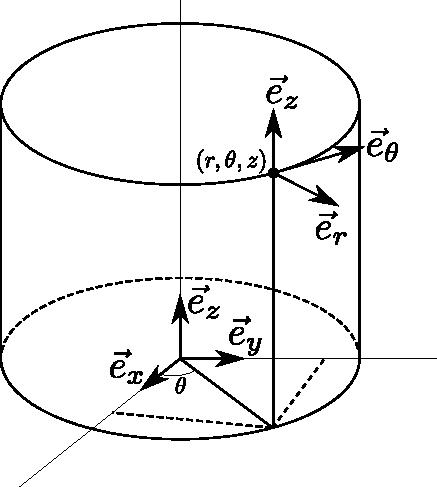
\includegraphics[width=.3\textwidth]{figures/cylindrical_coordinates}
  \caption{Cylindrical coordinate system spanned by $(\vec{e}_r, \vec{e}_\theta, \vec{e}_z)$.}
  \label{fig:cylindrical}
\end{figure}

\paragraph{Discretisation}

A discretised vector field $\vec{\phi}(\vec{x})$ reads
\begin{equation}
  \phi_r (\vec{x}) \vec{e}_r + \phi_\theta (\vec{x}) \vec{e}_\theta + \phi_z (\vec{x}) \vec{e}_z
  \approx
  \sum\limits_{m=1}^{n_\mathrm{nodes}}
  N^m (\vec{x}) \phi^{m}_{r}       \vec{e}_r      +
  N^m (\vec{x}) \phi^{m}_{\theta}  \vec{e}_\theta +
  N^m (\vec{x}) \phi^{m}_{z}       \vec{e}_z
\end{equation}
And consequently its discretised gradient reads
\begin{align}
  &\vec{\nabla} \vec{\phi} (\vec{x})
  \approx
  \sum\limits_{m=1}^{n_\mathrm{nodes}}
  \Bigg[
  \bigg(
  \vec{e}_r \frac{\partial}{\partial r} +
  \frac{1}{r} \vec{e}_\theta \frac{\partial}{\partial \theta} +
  \vec{e}_z \frac{\partial}{\partial z}
  \bigg)
  \bigg(
  N^m \phi^{m}_{r}       \vec{e}_r      +
  N^m \phi^{m}_{\theta}  \vec{e}_\theta +
  N^m \phi^{m}_{z}       \vec{e}_z
  \bigg)
  \Bigg]
  \\
  &=
  \sum\limits_{m=1}^{n_\mathrm{nodes}}
  \Bigg[
    \phi^{m}_{r     } \frac{\partial N^m}{\partial r} \vec{e}_r \vec{e}_r
  + \phi^{m}_{\theta} \frac{\partial N^m}{\partial r} \vec{e}_r \vec{e}_\theta
  + \phi^{m}_{z     } \frac{\partial N^m}{\partial r} \vec{e}_r \vec{e}_z
  \nonumber
  \\
  &\quad
  + \phi^{m}_{r     } \frac{1}{r} \frac{\partial N^m}{\partial \theta} \vec{e}_\theta \vec{e}_r
  + \phi^{m}_{r     } \frac{1}{r} N^m                                  \vec{e}_\theta \vec{e}_\theta
  + \phi^{m}_{\theta} \frac{1}{r} \frac{\partial N^m}{\partial \theta} \vec{e}_\theta \vec{e}_\theta
  - \phi^{m}_{\theta} \frac{1}{r} N^m                                  \vec{e}_r      \vec{e}_\theta
  + \phi^{m}_{z     } \frac{1}{r} \frac{\partial N^m}{\partial \theta} \vec{e}_\theta \vec{e}_z
  \nonumber
  \\
  &\quad
  + \phi^{m}_{r     } \frac{\partial N^m }{\partial z} \vec{e}_z \vec{e}_r
  + \phi^{m}_{\theta} \frac{\partial N^m }{\partial z} \vec{e}_z \vec{e}_\theta
  + \phi^{m}_{z     } \frac{\partial N^m }{\partial z} \vec{e}_z \vec{e}_z
  \Bigg]
\end{align}
whereby the spatial dependence was not denoted, but naturally persists. The above can be denoted in short as
\begin{equation}
  \vec{\nabla} \vec{\phi} (\vec{x})
  \approx
  \sum\limits_{m=1}^{n_\mathrm{nodes}}
  \mathcal{B}_m (\vec{x}) \cdot \vec{\phi}_m
\end{equation}
where the non-zero components of the third order $\mathcal{B}_m$ read
\begin{alignat}{4}
  \mathcal{B}^{m}_{r      r      r     } &= \frac{\partial N^m}{\partial r} & \qquad
  \mathcal{B}^{m}_{r      \theta \theta} &= \frac{\partial N^m}{\partial r} - \frac{1}{r} N^m & \qquad
  \mathcal{B}^{m}_{r      z      z     } &= \frac{\partial N^m}{\partial r}
  \nonumber
  \\
  \mathcal{B}^{m}_{\theta r      r     } &= \frac{1}{r} \frac{\partial N^m}{\partial \theta} & \qquad
  \mathcal{B}^{m}_{\theta \theta \theta} &= \frac{1}{r} \frac{\partial N^m}{\partial \theta} & \qquad
  \mathcal{B}^{m}_{\theta z      z     } &= \frac{1}{r} \frac{\partial N^m}{\partial \theta} & \qquad
  \mathcal{B}^{m}_{\theta \theta r     } &= \frac{1}{r} N^m
  \nonumber
  \\
  \mathcal{B}^{m}_{z      r      r     } &= \frac{\partial N^m}{\partial z} & \qquad
  \mathcal{B}^{m}_{z      \theta \theta} &= \frac{\partial N^m}{\partial z} & \qquad
  \mathcal{B}^{m}_{z      z      z     } &= \frac{\partial N^m}{\partial z}
\end{alignat}

\paragraph{Jacobian}

A Jacobian $\bm{J}$ can be defined to change coordinates as follows
\begin{equation}
  \vec{\nabla}_\xi = \bm{J} \cdot \vec{\nabla}
\end{equation}
which in components reads
\begin{equation}
  \vec{e}_\xi  \frac{\partial}{\partial \xi }  +
  \vec{e}_\eta \frac{\partial}{\partial \eta} +
  \vec{e}_\mu  \frac{\partial}{\partial \mu}
  =
  \bm{J} \cdot
  \left(
              \vec{e}_r      \frac{\partial}{\partial r     } +
  \frac{1}{r} \vec{e}_\theta \frac{\partial}{\partial \theta} +
              \vec{e}_z      \frac{\partial}{\partial z     }
  \right)
\end{equation}
The Jacobian is then obtained as
\begin{align}
  \bm{J}
  &=
  \vec{e}_\xi    \frac{\partial r     }{\partial \xi } \vec{e}_r      +
  \vec{e}_\xi  r \frac{\partial \theta}{\partial \xi } \vec{e}_\theta +
  \vec{e}_\xi    \frac{\partial z     }{\partial \xi } \vec{e}_z
  \nonumber
  \\
  &+
  \vec{e}_\eta   \frac{\partial r     }{\partial \eta} \vec{e}_r      +
  \vec{e}_\eta r \frac{\partial \theta}{\partial \eta} \vec{e}_\theta +
  \vec{e}_\eta   \frac{\partial z     }{\partial \eta} \vec{e}_z
  \nonumber
  \\
  &+
  \vec{e}_\mu    \frac{\partial r     }{\partial \mu } \vec{e}_r      +
  \vec{e}_\mu  r \frac{\partial \theta}{\partial \mu } \vec{e}_\theta +
  \vec{e}_\mu    \frac{\partial z     }{\partial \mu } \vec{e}_z
\end{align}

\paragraph{Axisymmetric}

Assuming axisymmetry implies assuming that there can be no variations along the $\vec{e}_\theta$ direction. This implies that any derivate $\partial / \partial \theta = 0$ and consequently that there are no degrees-of-freedom in the $\theta$ direction, i.e.\ $u_\theta = 0$. This implies that the only relevant non-zero components of the third order $\mathcal{B}_m$ read
\begin{alignat}{4}
  \mathcal{B}^{m}_{r      r      r     } &= \frac{\partial N^m}{\partial r} & \qquad
  \mathcal{B}^{m}_{r      z      z     } &= \frac{\partial N^m}{\partial r}
  \nonumber
  \\
  \mathcal{B}^{m}_{\theta \theta r     } &= \frac{1}{r} N^m
  \nonumber
  \\
  \mathcal{B}^{m}_{z      r      r     } &= \frac{\partial N^m}{\partial z} & \qquad
  \mathcal{B}^{m}_{z      z      z     } &= \frac{\partial N^m}{\partial z}
\end{alignat}
The Jacobian is furthermore reduced to
\begin{align}
  \bm{J}
  &=
  \vec{e}_\xi    \frac{\partial r     }{\partial \xi } \vec{e}_r +
  \vec{e}_\xi    \frac{\partial z     }{\partial \xi } \vec{e}_z
  \nonumber
  \\
  &+
  \vec{e}_\eta   \frac{\partial r     }{\partial \eta} \vec{e}_r +
  \vec{e}_\eta   \frac{\partial z     }{\partial \eta} \vec{e}_z
\end{align}

% \bibliography{example_refs}

\end{document}
